\documentclass[../report.tex]{subfiles}

\begin{document}
\section{Reformat OpenAlex Object and Create Neo4j Nodes}
\hspace{0.5cm} After getting the accurate faculty data, we can import them into graph database Neo4j to analyze the relationship between elements. Here's what I did at the beginning of the research: reformatting OpenAlex object and loading them into Neo4j. 
\par OpenAlex contains different types of nodes including: work, author, concept, funder, institution, publication and source. And these types are linked with certain properties. For example, work nodes are connected to author nodes with the ``authorship'' property in work node. In order to import these nodes into Neo4j, we need to reformat the OpenAlex object and create nodes with the corresponding properties. The original OpenAlex object is a multiple-level json file. Then I extract the important properties and flatten the object into single-level python dictionary, which is suitable for transforming to csv and loading into Neo4j. 

\begin{figure}[htbp]
    \centering
    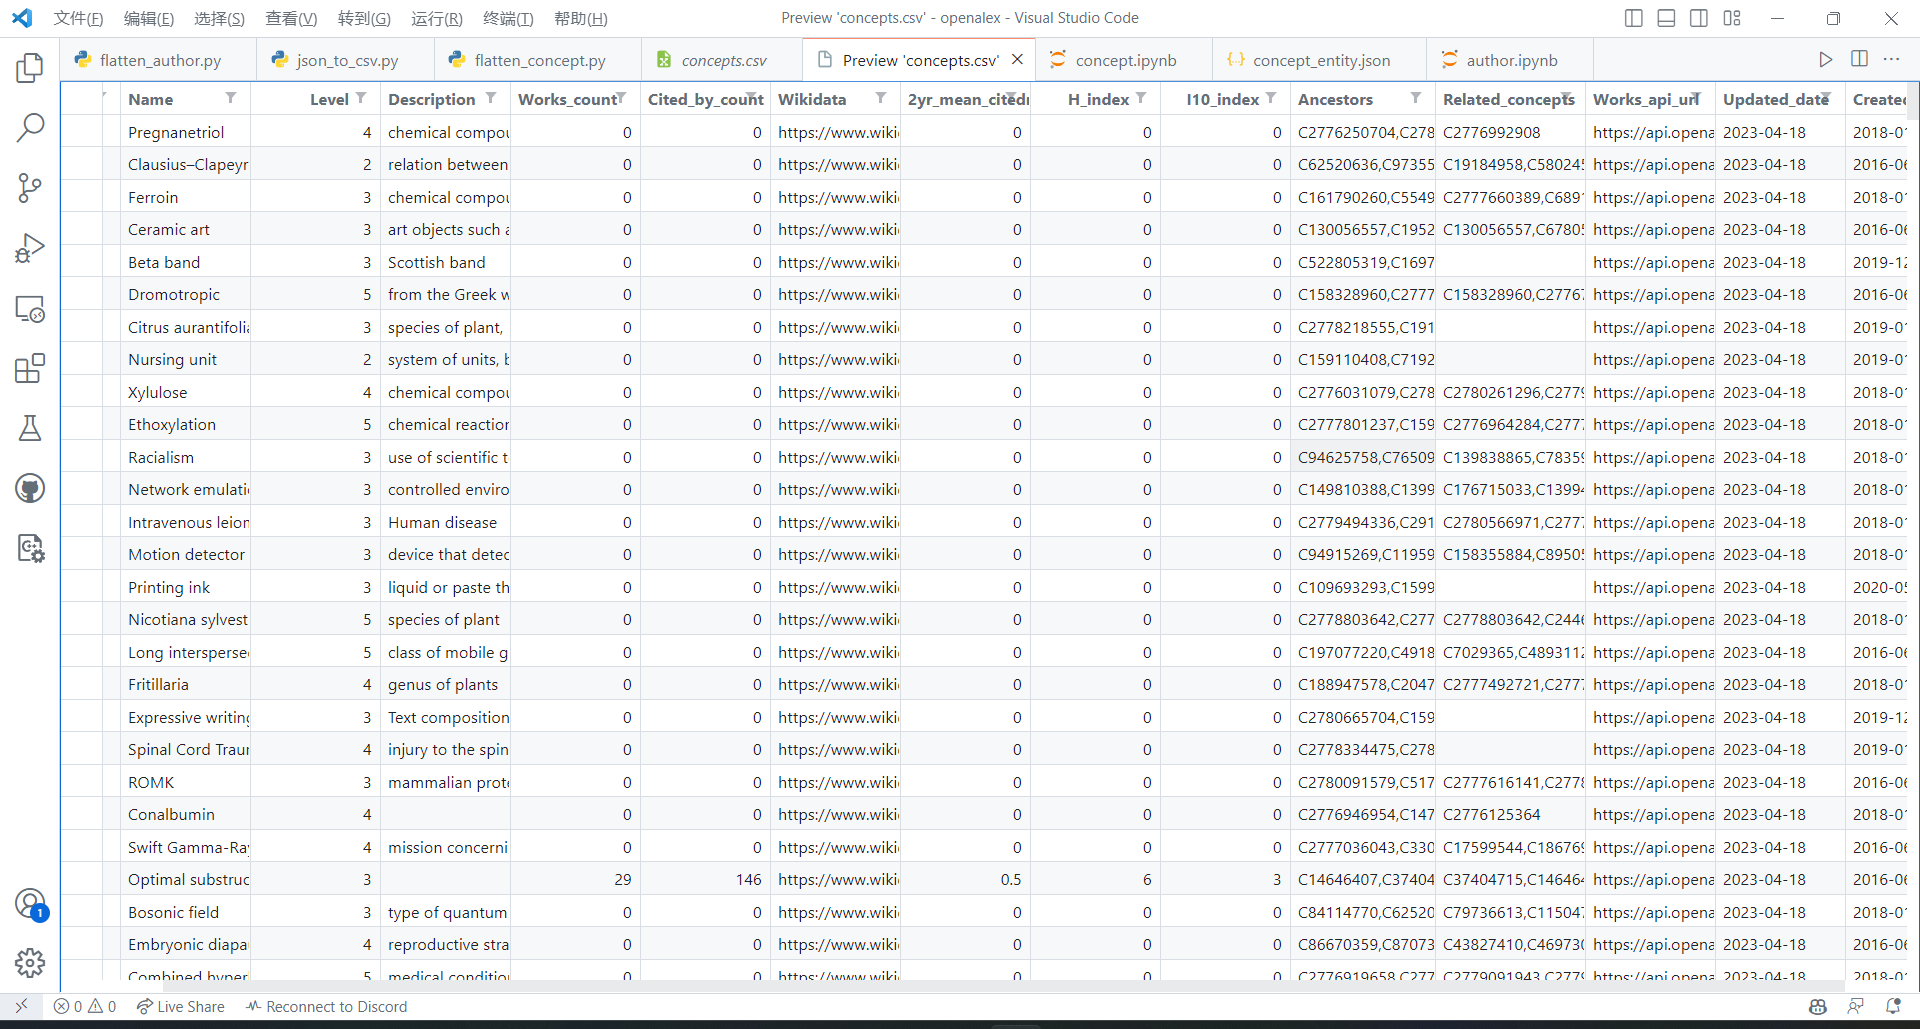
\includegraphics[width=1\textwidth]{./figs/reformat_example.png}
    \caption{Concept Nodes After Reformatting}
    \label{reformat_example}
  \end{figure}

\hspace{0.5cm} After getting the reformatted csv, we needs to create nodes in Neo4j using LOAD CSV tool.(\url{https://neo4j.com/developer/guide-import-csv/}) I classify the properties into self-property and relationship-property. Self-property is the property of the node itself, for example, the name of the author. Relationship-property is the property of the relationship between two nodes, for example, the authorship property between author and work. Then I create nodes with self-property and create relationships with relationship-property. The following figures show the final graph result.

\begin{figure}[htbp]
    \centering
    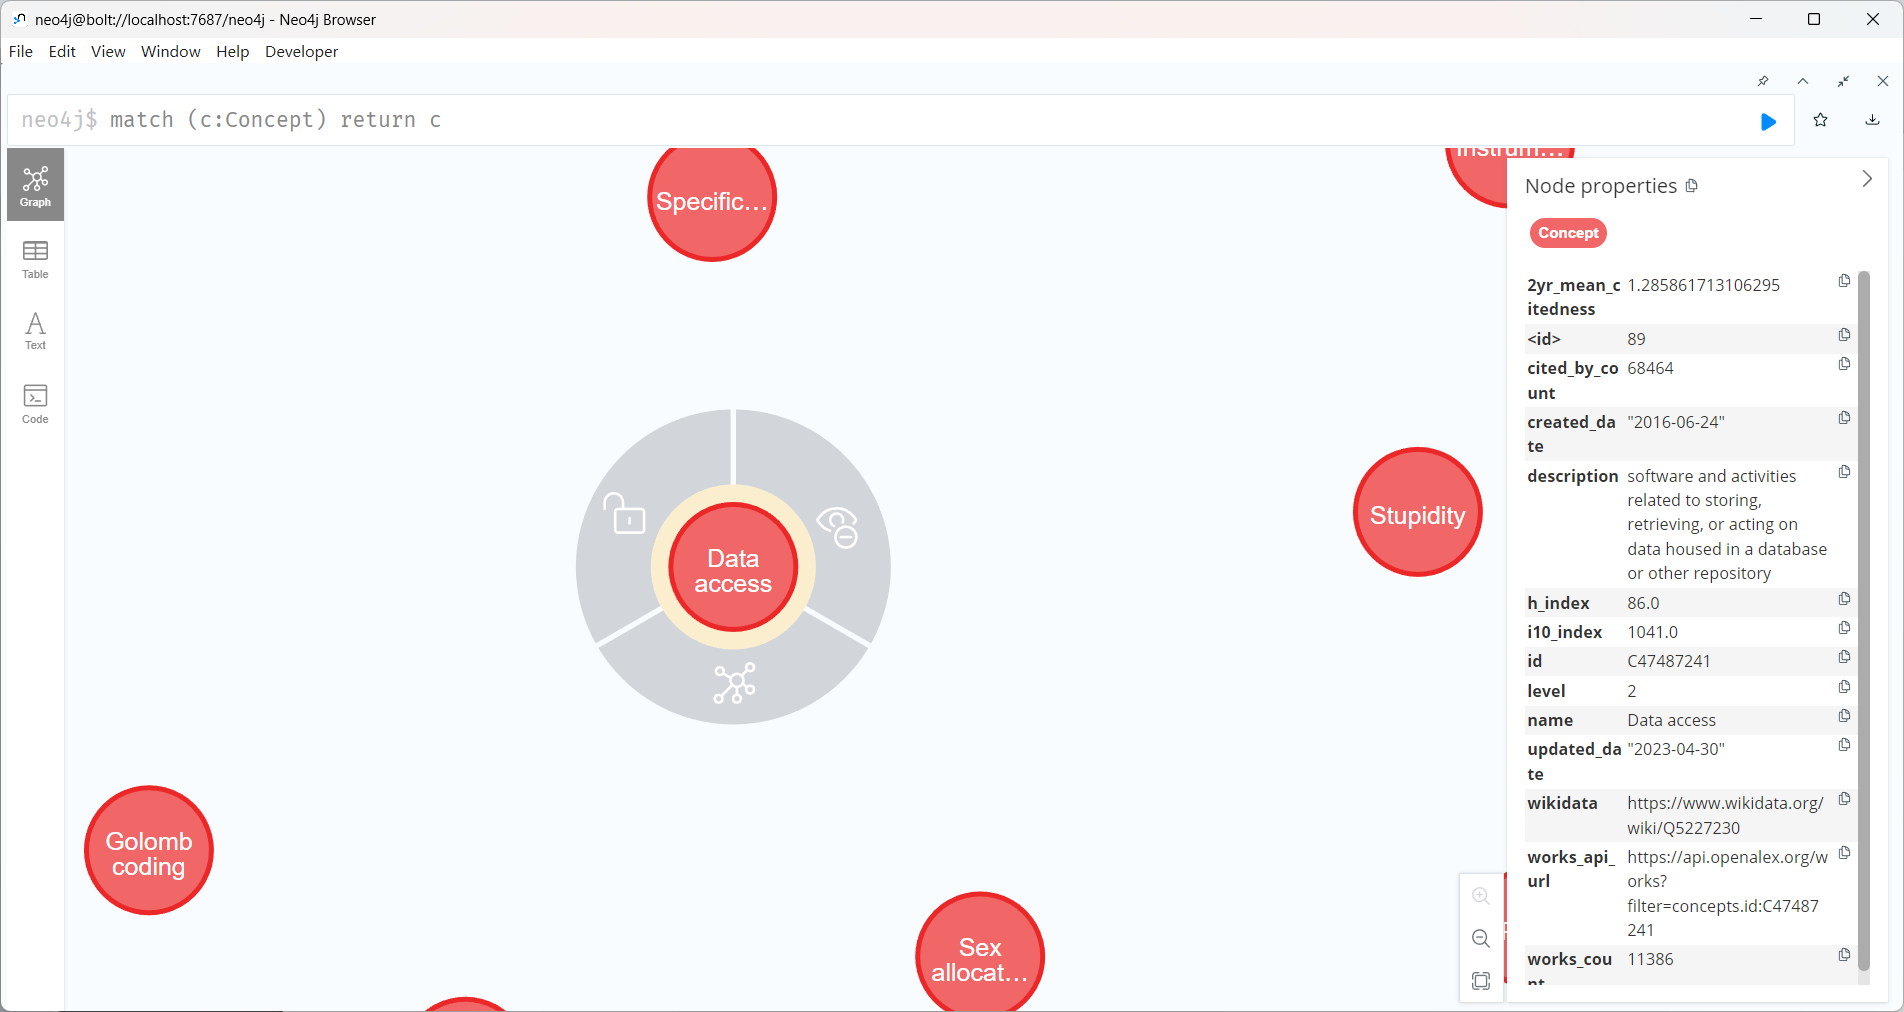
\includegraphics[width=1\textwidth]{./figs/concept_node.png}
    \caption{Concept Node Example in Neo4j}
    \label{concept_node}
  \end{figure}

  \begin{figure}[htbp]
    \centering
    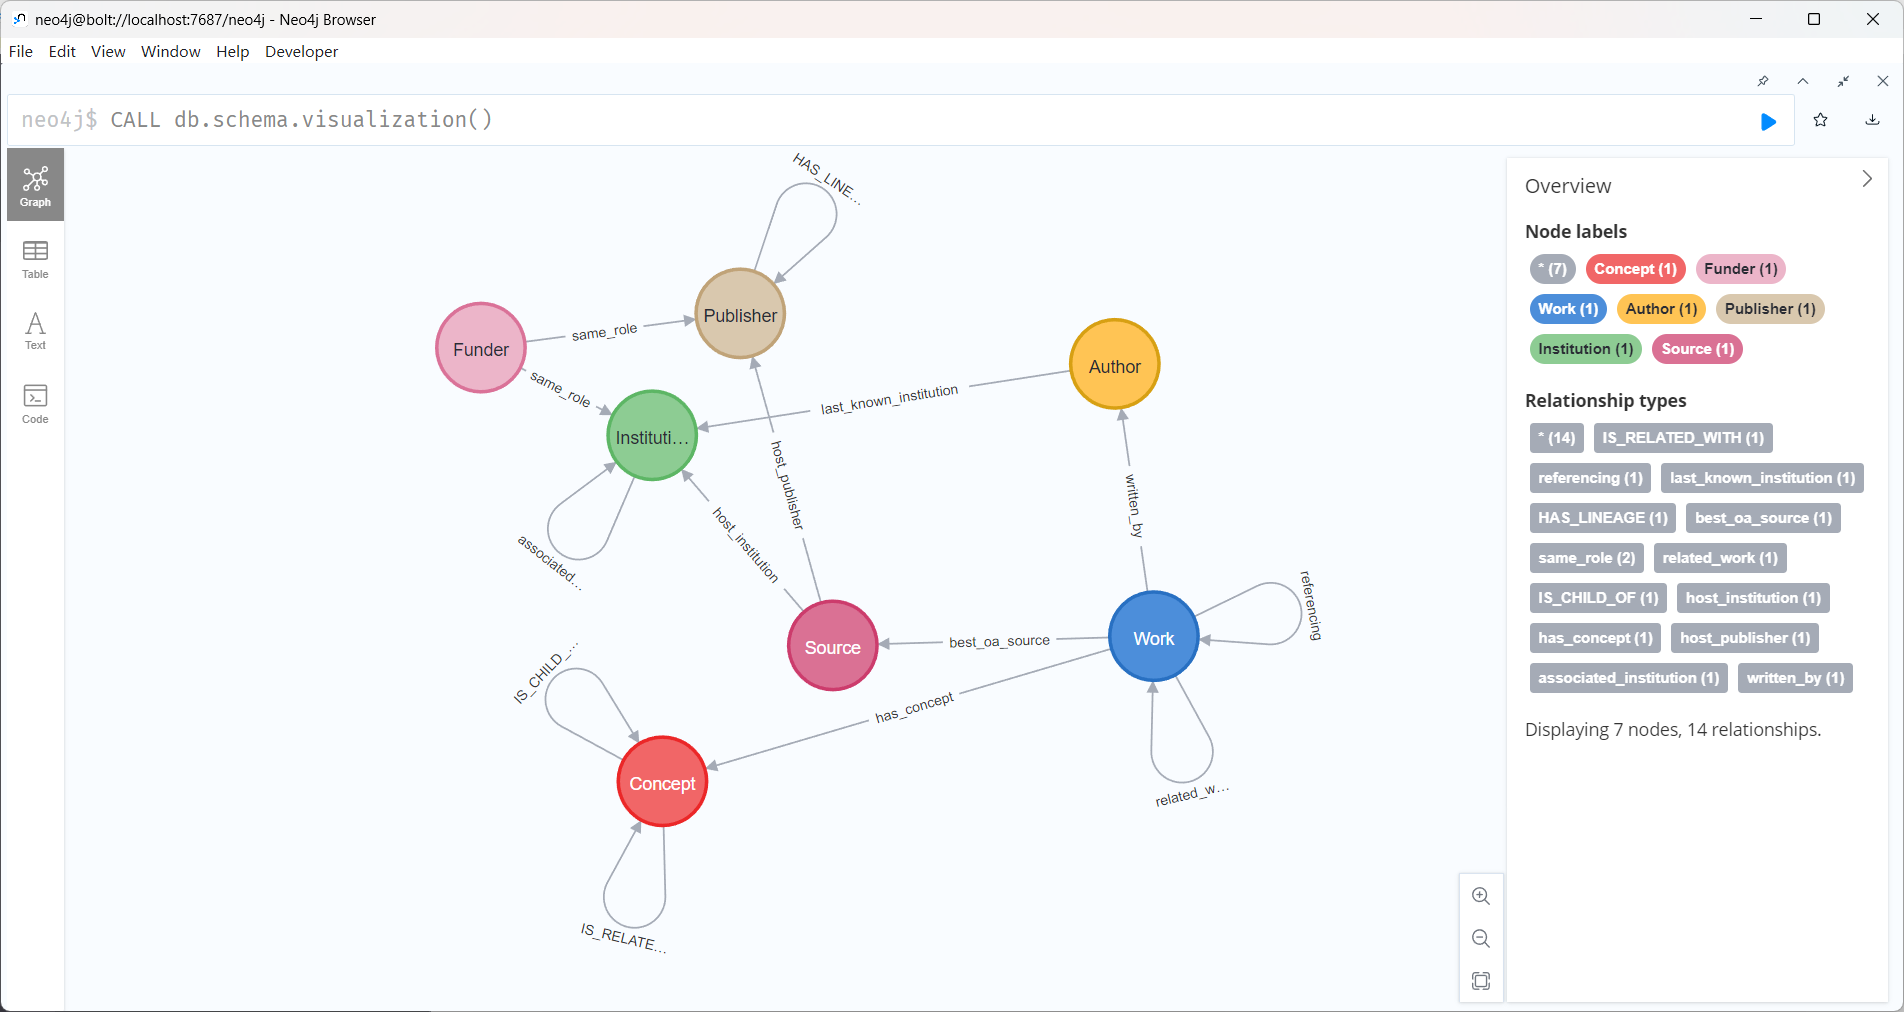
\includegraphics[width=1\textwidth]{./figs/schema.png}
    \caption{Schema of the Graph}
    \label{schema}
  \end{figure}
\newpage

\end{document}
